\section{Trazado de Conos con Vóxeles} % (fold)
\label{sec:trazado_de_conos}
El trazado de conos es utilizado para distintos aspectos visuales de la aplicación. En nuestra implementación este proceso se realiza durante el cálculo de iluminación utilizando sombreado diferido (sección \ref{sub:deferred_rendering_theory}). Utilizar sombreado diferido muy conveniente ya que durante el cálculo de iluminación solo necesario trazar conos sobre cada pixel en vez de cada fragmento incluyendo no visibles.

Como se menciona en la sección \ref{sec:trazado_de_conos_con_voxeles}. El trazado de conos es similar a ray-marching con la única diferencia que el volumen a muestrear incrementa de tamaño según la distancia recorrida. Esto es producto de la expansión de la apertura del cono a través de su distancia recorrida. Las muestras de mayor tamaño se obtienen utilizando los niveles de mip map descritos en la sección anterior.

Al utilizar vóxeles anisótropos se necesita saber que volúmenes direccionales van a ser utilizados para muestrear a través del recorrido del cono. Esto se determina según el signo de cada eje del vector direccional del cono. También es necesario calcular el peso de cada eje para obtener un resultado ponderado entre los tres volúmenes:
\\
\begin{lstlisting}[caption={Lógica para determinar volúmenes direccionales a utilizar durante el trazado de conos y peso por eje.}, label=Trace0]
vec4 TraceCone(vec3 position, vec3 normal, vec3 direction, float aperture)
{
    uvec3 visibleFace;
    visibleFace.x = (direction.x < 0.0) ? 0 : 1;
    visibleFace.y = (direction.y < 0.0) ? 2 : 3;
    visibleFace.z = (direction.z < 0.0) ? 4 : 5;
    // weight per axis for aniso sampling
    vec3 weight = direction * direction;
(*@\centerline{\raisebox{-1pt}[0pt][0pt]{$\vdots$}}@*)
}
\end{lstlisting}

Durante el recorrido del cono se utiliza la función de GLSL \emph{textureLod}. Esta función tiene como entrada una textura, una coordenada y un nivel mip. Durante la marcha del cono el nivel mip se obtiene del diámetro del cono dado una distancia desde el origen:
\begin{equation}
	V_{level} = \log_2(\frac{d}{V_{size}})
\end{equation}
Donde $d$ es el diámetro del círculo del cono según la distancia recorrida y $V_{size}$ es el tamaño de un vóxel en la cuadricula de vóxeles en el máximo nivel de detalle. El valor de $d$ se puede obtener de la siguiente ecuación:
\begin{equation}
	d = 2t\cdot\tan(\frac{\theta}{2})
\end{equation}
Donde $t$ es la distancia recorrida por el cono desde el punto de origen y $\theta$ es el ángulo de apertura del cono. En la siguiente figura podemos observar una representación visual de este recorrido:
\begin{figure}[H]
	\centering
	\captionsetup{justification=centering}
	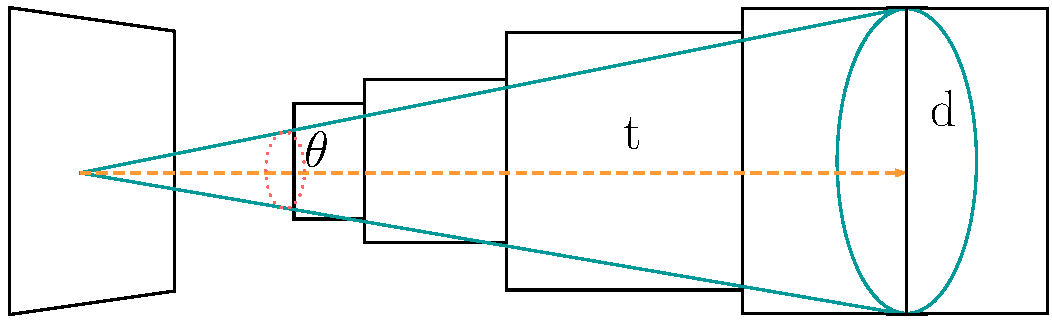
\includegraphics[width=.9\linewidth]{media/cone.pdf}
	\caption{Visualizacion del recorrido de un cono.}
\end{figure}

En nuestra implementación el punto de origen del cono es trasladado según el tamaño de un vóxel. Esto se hace para evitar que el cono colisione con el vóxel de origen:
\\
\begin{lstlisting}[caption={Traslado de origen del cono.}, label=Trace1]
vec4 TraceCone(vec3 position, vec3 normal, vec3 direction, float aperture)
{
(*@\centerline{\raisebox{-1pt}[0pt][0pt]{$\vdots$}}@*)
	// move further to avoid self collision
	float dst = voxelWorldSize;
	vec3 startPosition = position + normal * dst;
(*@\centerline{\raisebox{-1pt}[0pt][0pt]{$\vdots$}}@*)
}
\end{lstlisting}
Finalmente se comienza el trazado del cono a través de la escena:
\\
\begin{lstlisting}[caption={Trazado de cono con voxeles.}, label=Trace2]
layout(binding = 7) uniform sampler3D voxelTex;
layout(binding = 8) uniform sampler3D voxelTexMipmap[6];

vec4 AnistropicSample(vec3 coord, vec3 weight, uvec3 face, float lod)
{
    // anisotropic volumes level
    float anisoLevel = max(lod - 1.0f, 0.0f);
    // directional sample
    vec4 anisoSample = weight.x * textureLod(voxelTexMipmap[face.x], coord, anisoLevel)
                     + weight.y * textureLod(voxelTexMipmap[face.y], coord, anisoLevel)
                     + weight.z * textureLod(voxelTexMipmap[face.z], coord, anisoLevel);
    // linearly interpolate on base level
    if(lod < 1.0f)
    {
        vec4 baseColor = texture(voxelTex, coord);
        anisoSample = mix(baseColor, anisoSample, clamp(lod, 0.0f, 1.0f));
    }

    return anisoSample;                    
}
vec4 TraceCone(vec3 position, vec3 normal, vec3 direction, float aperture)
{
(*@\centerline{\raisebox{-1pt}[0pt][0pt]{$\vdots$}}@*)
    // final results
    vec4 coneSample = vec4(0.0f);
    float maxDistance = maxTracingDistanceGlobal / voxelScale

    while(coneSample.a < 1.0f && dst <= maxDistance)
    {
        vec3 conePosition = startPosition + direction * dst;
        // cone expansion and respective mip level based on diameter
        float diameter = 2.0f * aperture * dst;
        float mipLevel = log2(diameter / voxelWorldSize);
        // convert position to texture coord
        vec3 coord = WorldToVoxel(conePosition);
        // get directional sample from anisotropic representation
        vec4 anisoSample = AnistropicSample(coord, weight, visibleFace, mipLevel);
        // front to back composition
        coneSample += (1.0f - coneSample.a) * anisoSample;
        // move further into volume
        dst += diameter * samplingFactor;
    }

    return coneSample;
}
\end{lstlisting}
En el método \emph{AnistropicSample} se puede observar el muestreo direccional, ponderado por el peso de cada eje en la dirección del cono y el uso de la función \emph{mix()} para interpolar entre los volúmenes direccionales y la textura base. 

Durante el trazado se observa cómo se obtiene la posición del cono según la distancia recorrida y el uso de las operaciones ya mencionadas para obtener el diámetro y el nivel mip. La función \emph{WorldToVoxel} aparece para cambiar una posición en espacio de mundo a espacio de textura como fue mencionado para el algoritmo \ref{SpaceTransform}. La distancia recorrida es alterada por una variable \emph{samplingFactor} esto permite disminuir la distancia entre muestreos para lograr resultados más suaves con un costo en rendimiento.

Para acumular los valores muestreados través del recorrido del cono se utiliza acumulación volumétrica \emph{front-to-back}. Para esto es necesario llevar pista de un valor oclusión $a$ y color $c$. La actualización de estos valores por cada paso se realiza de la siguiente manera: $c=c+(1-a)c_2$ y $a=a+(1-a)a_2$. En el algoritmo se puede observar que esto se realiza con la variable \emph{coneSample}.

\subsection{Reflexion Difusa} % (fold)
\label{sub:reflexion_difuse}
Para el cálculo de reflexión difusa se utilizan seis conos dentro de la semiesfera orientada por el vector normal como se describen en la figura \ref{fig:brdf_cones2}. El código para la integración de estos conos es el siguiente:
\\
\begin{lstlisting}[caption={Conos para reflexion difusa.}, label=Trace3]
const vec3 diffuseConeDirections[] =
{
    vec3(0.0f, 1.0f, 0.0f),
    vec3(0.0f, 0.5f, 0.866025f),
    vec3(0.823639f, 0.5f, 0.267617f),
    vec3(0.509037f, 0.5f, -0.7006629f),
    vec3(-0.50937f, 0.5f, -0.7006629f),
    vec3(-0.823639f, 0.5f, 0.267617f)
};
const float diffuseConeWeights[] =
{
    PI / 4.0f,
    3.0f * PI / 20.0f,
    3.0f * PI / 20.0f,
    3.0f * PI / 20.0f,
    3.0f * PI / 20.0f,
    3.0f * PI / 20.0f,
};
vec4 CalculateIndirectLighting(vec3 position, vec3 normal, vec3 albedo, vec4 specular)
{
    vec4 diffuseTrace = vec4(0.0f);
    vec3 coneDirection = vec3(0.0f);
(*@\centerline{\raisebox{-1pt}[0pt][0pt]{$\vdots$}}@*)
    // component greater than zero
    if(any(greaterThan(albedo, diffuseTrace.rgb)))
    {
        // diffuse cone setup
        const float aperture = 0.57735f // tan(60/2);
        vec3 guide = vec3(0.0f, 1.0f, 0.0f);

        if (abs(dot(normal,guide)) == 1.0f)
        {
            guide = vec3(0.0f, 0.0f, 1.0f);
        }

        // find a right and up vector
        vec3 right = normalize(guide - dot(normal, guide) * normal);
        vec3 up = cross(right, normal);

        for(int i = 0; i < 6; i++)
        {
            coneDirection = normal;
            coneDirection += diffuseConeDirections[i].x * right + diffuseConeDirections[i].z * up;
            coneDirection = normalize(coneDirection);
            // cumulative result
            diffuseTrace += TraceCone(position, normal, coneDirection, aperture) * diffuseConeWeights[i];
        }

        diffuseTrace.rgb *= albedo;
    }
(*@\centerline{\raisebox{-1pt}[0pt][0pt]{$\vdots$}}@*)
}
\end{lstlisting}
Las direcciones, pesos de integración y tangente del ángulo ya se encuentran pre-calculados. Para rotar a lo largo del vector normales se obtienen vectores direccionales perpendiculares a la normal utilizando un vector guía.
\subsection{Reflexion Especular} % (fold)
\label{sub:reflexion_especular}
La reflexión especular es un solo cono con la dirección del lóbulo especular y una apertura adecuada a la potencia especular de un material para la \ac{BRDF} Blinn-Phong. El código para el cono especular es el siguiente:
\\
\begin{lstlisting}[caption={Cono para reflexion especular.}, label=Trace4]
vec4 CalculateIndirectLighting(vec3 position, vec3 normal, vec3 albedo, vec4 specular)
{
    vec4 specularTrace = vec4(0.0f);
    vec3 coneDirection = vec3(0.0f);
(*@\centerline{\raisebox{-1pt}[0pt][0pt]{$\vdots$}}@*)
    // component greater than zero
    if(any(greaterThan(specular.rgb, specularTrace.rgb)))
    {
        vec3 viewDirection = normalize(cameraPosition - position);
        vec3 coneDirection = reflect(-viewDirection, normal);
        coneDirection = normalize(coneDirection);
        // specular cone setup, minimum of 1 grad, fewer can severly slow down performance
        float aperture = max(tan(HALF_PI * (1.0f - specular.a)), 0.0174533f);
        specularTrace = TraceCone(position, normal, coneDirection, aperture, false);
        specularTrace.rgb *= specular.rgb;
    }
(*@\centerline{\raisebox{-1pt}[0pt][0pt]{$\vdots$}}@*)
}
\end{lstlisting}
Para modular la apertura del cono especular utilizamos la función tangente. En el componente alfa de la especular se encuentra la potencia especular sin escalar, esto quiere decir que va de cero a uno. También limitamos el cono especular a mínimo un grado de apertura. Los conos extremadamente finos puede afectar mucho el rendimiento del programa, además de esto la apertura no puede ser cero.
\subsection{Oclusión Ambiental} % (fold)
\label{sub:oclusion_ambient}
En nuestra implementación los conos utilizados para calcular la reflexión difusa son utilizados para calcular la oclusión ambiental. Primero se realiza una pequeña adición a la función \emph{TraceCone} para incluir el cálculo de oclusión ambiental como es descrito en la sección \ref{sub:occl_ambt_prop}:
\\
\begin{lstlisting}[caption={Oclusión ambiental para el algoritmo de trazado de conos.}, label=Trace5]
vec4 TraceCone(vec3 position, vec3 normal, vec3 direction, float aperture, bool traceOcclusion)
{
(*@\centerline{\raisebox{-1pt}[0pt][0pt]{$\vdots$}}@*)
    // final results
    vec4 coneSample = vec4(0.0f);
    float maxDistance = maxTracingDistanceGlobal / voxelScale
   	float occlusion = 0.0f;
    float falloff = 0.5f * aoFalloff * voxelScale;

    while(coneSample.a < 1.0f && dst <= maxDistance)
    {
        vec3 conePosition = startPosition + direction * dst;
        // cone expansion and respective mip level based on diameter
        float diameter = 2.0f * aperture * dst;
        float mipLevel = log2(diameter / voxelWorldSize);
        // convert position to texture coord
        vec3 coord = WorldToVoxel(conePosition);
        // get directional sample from anisotropic representation
        vec4 anisoSample = AnistropicSample(coord, weight, visibleFace, mipLevel);
        // front to back composition
        coneSample += (1.0f - coneSample.a) * anisoSample;
        // ambient occlusion
        if(traceOcclusion && occlusion < 1.0)
        {
            occlusion += ((1.0f - occlusion) * anisoSample.a) / (1.0f + falloff * diameter);
        }
        // move further into volume
        dst += diameter * samplingFactor;
    }

    return vec4(coneSample.rgb, occlusion);
}
\end{lstlisting}
El trazado del cono ambiental es muy similar a la acumulación completa la diferencia es la multiplicación por la función $f(r)$ descrita en la sección \ref{sub:occl_ambt_prop} Acá nuestro $\lambda$ es la variable \emph{falloff} pre-multiplicada por $0.5$ para obtener el radio del cono. La oclusión ambiental es almacenada en el alfa del vector retornado por $TraceCone$ esta será utilizada luego para la composición final de la imagen.
% subsection oclusion_ambient (end)
% subsection reflexion_especular (end)
% subsection reflexion_difuse (end)
% section trazado_de_conos (end)
